% Additional styles
\tikzstyle{block} = [rectangle, draw, text width=8em, text centered, rounded corners, minimum height=4em, line width=4pt]
    
\tikzstyle{line} = [draw, -latex]



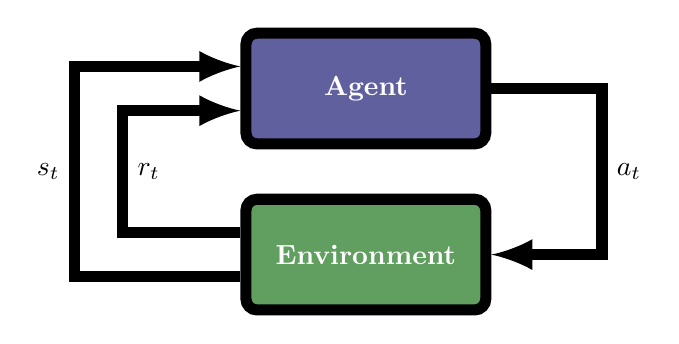
\begin{tikzpicture}[node distance = 6em, auto, thick]
    \node [block, fill=blue!25!gray, text=white] (Agent) {\textbf{Agent}};
    \node [block, below of=Agent, fill=green!25!gray, text=white] (Environment) {\textbf{Environment}};
    
     \path [line, line width=4pt] (Agent.0) --++ (4em,0em) |- node [near start]{$\boldsymbol{a_t}$} (Environment.0);
     \path [line, line width=4pt] (Environment.190) --++ (-6em,0em) |- node [near start] {$\boldsymbol{s_t}$} (Agent.170);
     \path [line, line width=4pt] (Environment.170) --++ (-4.25em,0em) |- node [near start, right] {$\boldsymbol{r_t}$} (Agent.190);
\end{tikzpicture}